\begin{enumerate}[label=\thesection.\arabic*.,ref=\thesection.\theenumi]
\numberwithin{equation}{enumi}
\item For a unity feedback system shown in Fig. \ref{fig:ee17btech11031_tiklap_ke}
\begin{figure}[!ht]
    \centering
	\resizebox{\columnwidth}{!}{
\tikzstyle{block} = [draw, fill=blue!20, rectangle, 
    minimum height=1cm, minimum width=1cm]
\tikzstyle{sum} = [draw, fill=blue!20, circle, node distance=1cm]
\tikzstyle{input} = [coordinate]
\tikzstyle{output} = [coordinate]
\tikzstyle{pinstyle} = [pin edge={to-,thin,black}]

% The block diagram code is probably more verbose than necessary
\begin{tikzpicture}[auto, node distance=2cm,>=latex']
    % We start by placing the blocks
    \node [input, name=input] {};
    \node [sum, right of=input] (sum) {};
    \node [block, right of=sum] (controller) {G(s)};
    \node [output, right of=controller, node distance = 3cm] (output) {};
    \node [block, below of=controller] (measurements) {1};
    % We draw an edge between the controller and system block to 
    % calculate the coordinate u. We need it to place the measurement block. 
    % Once the nodes are placed, connecting them is easy. 
    \draw [draw,->] (input) -- node {$R(s)$} (sum);
    \draw [->] (sum) -- node {} (controller);
    \draw [->] (controller) -- node[name=y] {$Y(s)$} (output);
    \draw [->] (y) |- node {} (measurements);
    \draw [->] (measurements) -| node[pos=0.99] {$-$} node[near end] {} (sum);
\end{tikzpicture}

}
    \caption{}
    \label{fig:ee17btech11031_tiklap_ke}
\end{figure}
\begin{align}
    G\brak{s} = \frac{K}{s\brak{s+1}}
    \label{eq:ee17btech11031_system1}
\end{align}
Design a PD controller such that the phase margin is 45\degree and appropriate steady state error is less than or equal to $\frac{1}{15}$ units of the final output value. Further the gain crossover frequency of the system must be less than 7.5 rad/s.

\solution Using TABLE \ref{table:ee18btech11021}
% The above Table is referred from other's person question.By giving input to ee18btech11021.tex in gvv_control_mannual, table number will be visible. % 
The gain after cascading the PD controller with G\brak{s} is
\begin{align}
    G_{c}\brak{s} = \frac{K_{P}\brak{1 + T_{d}s}K}{s\brak{s+1}}
    \label{eq:ee17btech11031_fir}
\end{align}

\begin{table}[!ht]
    \centering
    \input{./table/ee17btech11031_t_ke.tex}
    \caption{System Types and Poles at Origin}
    \label{table:ee17btech11031_t_ke}
\end{table}


Using TABLE \ref{table:ee17btech11031_t_ke}, \eqref{eq:ee17btech11031_fir} is Type 1 system.
\begin{align}
    e_{ss} = \frac{1}{\lim_{s \to 0} sG_{c}\brak{s}}\\
    e_{ss} \leq \frac{1}{15} \lim_{s \to 0} sG_{c}\brak{s}\\
    \implies K_{P}K \geq \sqrt{15}
\end{align}

For Phase Margin 45\degree, at gain crossover frequency $\omega$,

\begin{align}
    \tan^{-1}\brak{T_{d}\omega} - \tan^{-1}\brak{\omega} = -45 \degree\\
    \abs{G_{c}\brak{\j\omega}} = \frac{\sqrt{15}\sqrt{T_{d}^2\omega^2 + 1}}{\omega\sqrt{\omega^2+1}} = 1
\end{align}
By Hit and Trial, one of the best combinations is
\begin{align}
    \omega = 2.893\\
    T_{d} = -0.71
\end{align}

\begin{table}[!ht]
    \centering
    \input{./table/ee17btech11031_final_ke.tex}
    \caption{}
    \label{table:ee17btech11031_final}
\end{table}

\item
Verify using a Python Plot

\solution The following code plots Fig. \ref{fig:ee17btech11031_pd_ke}

\begin{lstlisting}
codes/ee17btech11031_pd_ke.py
\end{lstlisting}

\begin{figure}[!ht]
\centering
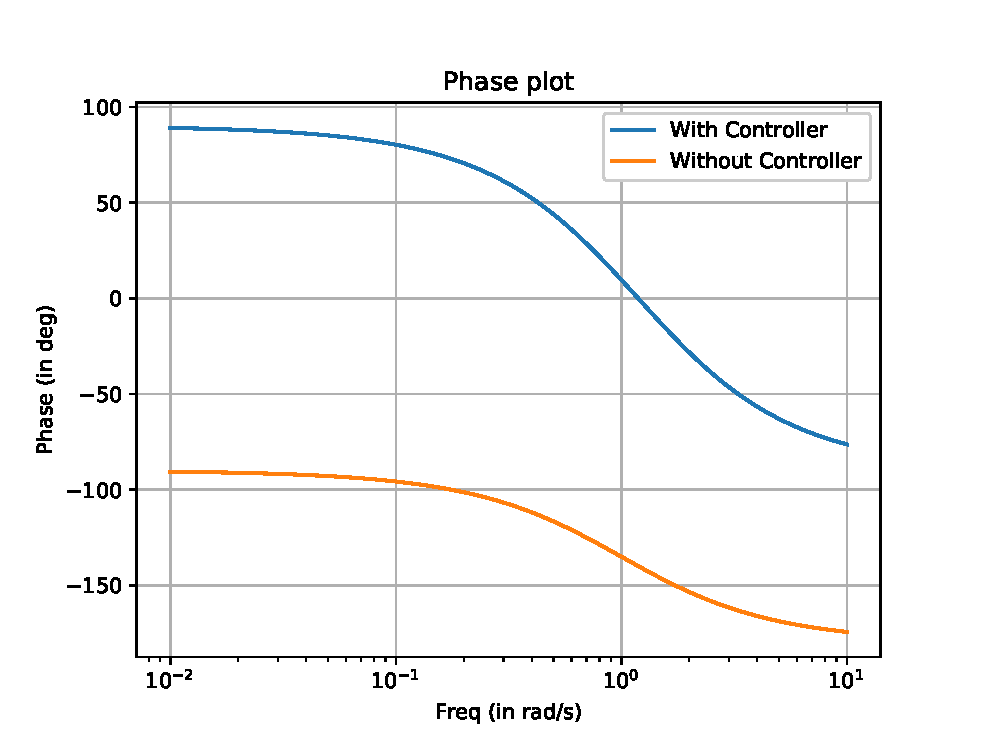
\includegraphics[width=\columnwidth]{./figs/ee17btech11031_pd_ke.eps}
\caption{}
\label{fig:ee17btech11031_pd_ke}
\end{figure}
\end{enumerate}
